\chapter{Complexação}\label{ch:b1:complexation}

Despeje um pouco de solução de amônia em sulfato de cobre(II) azul-claro:
forma-se imediatamente um precipitado azul-claro. Despeje mais, e o
precipitado se dissolve em uma solução de um azul profundo, quase cor de
tinta. Nada nos capítulos de ácido--base ou de precipitação explica a
segunda etapa. As moléculas de amônia se ligaram ao íon cobre por seus
\omterm{def:b1:lewis-resonance-vsepr:lewis}{pares não ligantes} e formaram uma nova espécie, um \omterm{def:b1:complexation:complex}{complexo}, mais
estável que o hidróxido e de outra cor. Os \omterm{def:b1:complexation:complex}{complexos} transportam o
oxigênio no sangue, prendem o metal na clorofila e na vitamina B$_{12}$,
amolecem a água dura e dissolvem metais que nada mais dissolve. Este
capítulo os trata como mais uma troca de partículas em água, com suas
próprias constantes e seus próprios diagramas.

\begin{recall}
Os \omterm{def:b1:lewis-resonance-vsepr:lewis-acid}{ácidos de Lewis} (aceptores de par de elétrons), as \omterm{def:b1:lewis-resonance-vsepr:lewis-acid}{bases de Lewis}
(doadoras de par de elétrons) e a \omterm{def:b1:lewis-resonance-vsepr:lewis-acid}{ligação dativa} foram definidos no
\cref{ch:b1:lewis-resonance-vsepr}. Os \omterm{def:b1:predominant-reaction:predominance}{diagramas de predominância} e o
método da \omterm{def:b1:predominant-reaction:predominant-reaction}{reação predominante} vêm do \cref{ch:b1:predominant-reaction};
o \omterm{def:b1:precipitation:solubility-product}{produto de solubilidade} e a condição de precipitação, do
\cref{ch:b1:precipitation}.
\end{recall}

\begin{omfigure}
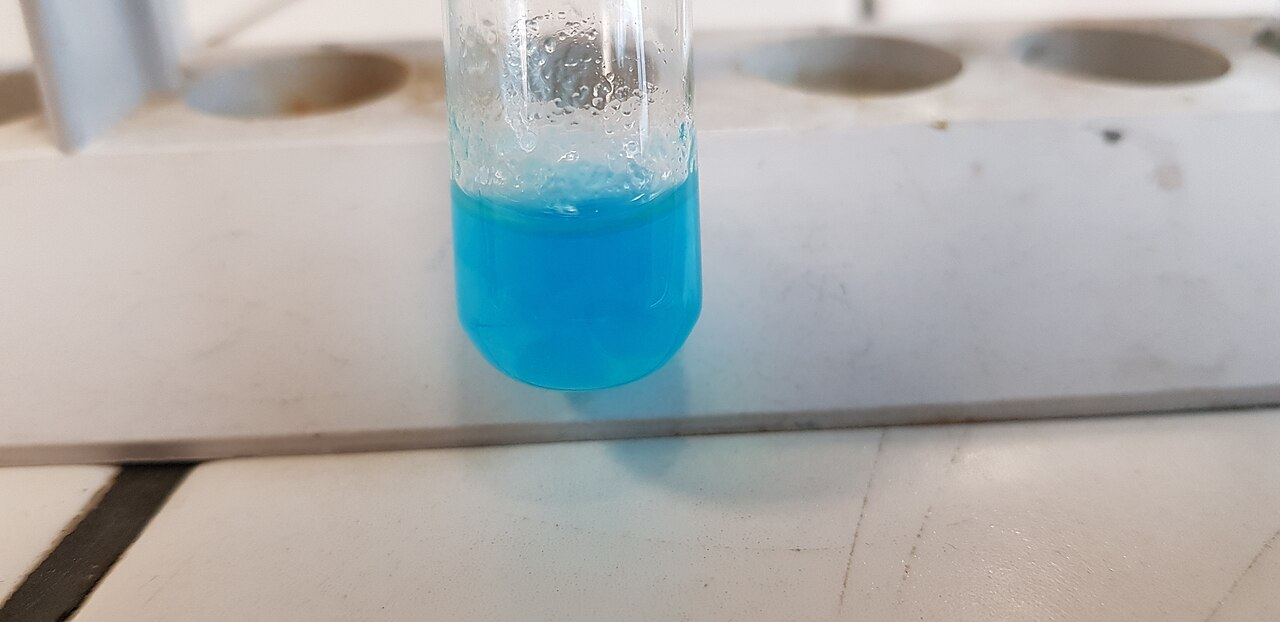
\includegraphics[height=4.2cm]{images/book2/copper-hydroxide.jpg}\hspace{0.6em}%
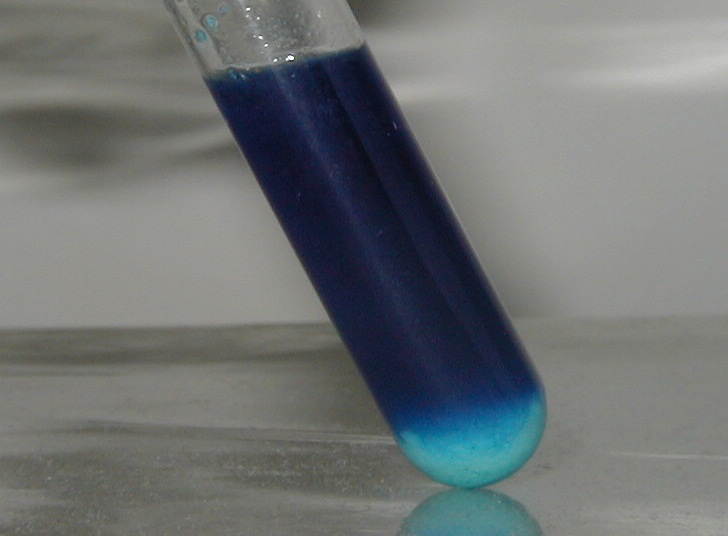
\includegraphics[height=4.2cm]{images/book2/copper-ammine.jpg}

{\small À esquerda: uma suspensão de hidróxido de cobre(II) azul-claro
(fotografia de Alvy16, CC BY 4.0). À direita: com mais amônia, o sólido
se dissolve no íon tetra-aminocobre(II), azul profundo; um pouco de
hidróxido não dissolvido ainda está no fundo do tubo (fotografia de
Chemicalinterest, domínio público). Ambas da Wikimedia Commons.}
\end{omfigure}

\section{Complexos e ligantes}

\begin{definition}[Complexo, átomo central, ligante]\label{def:b1:complexation:complex}
Um \emph{complexo}\index{complexo} é uma espécie formada por um
\emph{átomo central}\index{atomo central@átomo central} ou íon central, em geral um cátion
metálico que atua como \omterm{def:b1:lewis-resonance-vsepr:lewis-acid}{ácido de Lewis}, ligado por \omterm{def:b1:lewis-resonance-vsepr:lewis-acid}{ligações dativas} a
moléculas ou íons que atuam como \omterm{def:b1:lewis-resonance-vsepr:lewis-acid}{bases de Lewis}, os
\emph{ligantes}\index{ligante}. Sua fórmula é escrita entre colchetes,
com sua carga total: $[\ce{Cu(NH3)4}]^{2+}$,
$[\ce{Fe(CN)6}]^{4-}$, $[\ce{Ag(NH3)2}]^{+}$, $[\ce{FeSCN}]^{2+}$.
\end{definition}

A carga do \omterm{def:b1:complexation:complex}{complexo} é a soma das cargas do íon central e dos \omterm{def:b1:complexation:complex}{ligantes}:
$\mathrm{Fe^{2+}}$ e seis \ce{CN-} formam
$[\ce{Fe(CN)6}]^{4-}$. Um \omterm{def:b1:complexation:complex}{ligante} precisa de pelo menos um \omterm{def:b1:lewis-resonance-vsepr:lewis}{par não
ligante}: \ce{NH3}, \ce{H2O}, \ce{OH-}, \ce{Cl-}, \ce{CN-}, \ce{SCN-}
(ligado pelo S ou pelo N). Todo íon metálico em água já é, na verdade,
um \omterm{def:b1:complexation:complex}{complexo} com moléculas de água como \omterm{def:b1:complexation:complex}{ligantes},
$[\ce{Cu(H2O)6}]^{2+}$ ou $[\ce{Fe(H2O)6}]^{3+}$; formar outro \omterm{def:b1:complexation:complex}{complexo}
significa trocar essas moléculas de água por outros \omterm{def:b1:complexation:complex}{ligantes}, e os
\omterm{def:b1:complexation:complex}{ligantes} água são omitidos das fórmulas, assim como se escreve \ce{H3O+}
para o próton hidratado.
\begin{omfigure}
\begin{tikzpicture}[font=\small, line cap=round]
  % [Ag(NH3)2]+ : linear
  \begin{scope}
    \node (ag) at (0,0) {\ce{Ag}};
    \node (n1) at (-1.2,0) {\ce{H3N}};
    \node (n2) at (1.2,0) {\ce{NH3}};
    \draw[thick] (n1) -- (ag) -- (n2);
    \node at (0,-1.75) {$[\ce{Ag(NH3)2}]^{+}$, linear};
  \end{scope}
  % [Cu(NH3)4]2+ : square plane in perspective
  \begin{scope}[xshift=4.3cm, every node/.style={fill=white, inner sep=1.5pt}]
    \node (cu) at (0,0) {\ce{Cu}};
    \node (a) at (-1.45,-0.5) {\ce{H3N}};
    \node (b) at (1.45,0.5) {\ce{NH3}};
    \node (c) at (0.85,-0.9) {\ce{NH3}};
    \node (d) at (-0.85,0.9) {\ce{H3N}};
    \begin{pgfonlayer}{background}
    \draw[gray, dashed] (a.center) -- (c.center) -- (b.center) -- (d.center) -- cycle;
    \end{pgfonlayer}
    \draw[thick] (cu) -- (a); \draw[thick] (cu) -- (b);
    \draw[thick] (cu) -- (c); \draw[thick] (cu) -- (d);
    \node at (0,-1.75) {$[\ce{Cu(NH3)4}]^{2+}$, quadrado plano};
  \end{scope}
  % [Fe(CN)6]4- : octahedron
  \begin{scope}[xshift=9.2cm, every node/.style={fill=white, inner sep=1.5pt}]
    \node (fe) at (0,0) {\ce{Fe}};
    \node (t) at (0,1.3) {\ce{CN}};
    \node (u) at (0,-1.3) {\ce{CN}};
    \node (l) at (-1.45,-0.45) {\ce{NC}};
    \node (r) at (1.45,0.45) {\ce{CN}};
    \node (f) at (0.8,-0.8) {\ce{CN}};
    \node (k) at (-0.8,0.8) {\ce{NC}};
    \begin{pgfonlayer}{background}
    \draw[gray, dashed] (l.center) -- (f.center) -- (r.center) -- (k.center) -- cycle;
    \end{pgfonlayer}
    \foreach \x in {t,u,l,r,f,k} \draw[thick] (fe) -- (\x);
    \node at (0,-1.75) {$[\ce{Fe(CN)6}]^{4-}$, octaédrico};
  \end{scope}
\end{tikzpicture}

{\small Três \omterm{def:b1:complexation:complex}{complexos} e suas formas. Cada traço é uma \omterm{def:b1:lewis-resonance-vsepr:lewis-acid}{ligação dativa} do
\omterm{def:b1:lewis-resonance-vsepr:lewis}{par não ligante} do \omterm{def:b1:complexation:complex}{ligante} (o N da amônia, o C do cianeto) ao íon
metálico; as linhas tracejadas delimitam o quadrado de quatro \omterm{def:b1:complexation:complex}{ligantes}.
As formas dos \omterm{def:b1:complexation:complex}{complexos} são explicadas no volume do 2.º~ano.}
\end{omfigure}

\begin{definition}[Ligante polidentado, quelato]\label{def:b1:complexation:chelate}
Um \omterm{def:b1:complexation:complex}{ligante} que se liga ao mesmo íon central por vários de seus átomos ao
mesmo tempo é um \emph{ligante polidentado}\index{ligante polidentado}; o
\omterm{def:b1:complexation:complex}{complexo} que ele forma, no qual o \omterm{def:b1:complexation:complex}{ligante} fecha anéis em torno do íon
metálico, é um \emph{quelato}\index{quelato}. A etilenodiamina
\ce{H2N-CH2-CH2-NH2} se liga por dois átomos de N, o íon oxalato
\ce{C2O4^2-} por dois átomos de O, e o íon etilenodiaminotetra-acetato
(\emph{edta}, escrito \ce{Y^4-}) por dois átomos de N e quatro de O.
\end{definition}

\begin{omfigure}
\setchemfig{atom sep=1.9em}
\chemfig{N(-[3]-[2]C(=[1]O)-[3]O^{-})(-[5]-[6]C(=[7]O)-[5]O^{-})-[0]-[0]N(-[1]-[2]C(=[3]O)-[1]O^{-})(-[7]-[6]C(=[5]O)-[7]O^{-})}
\hspace{2.2em}
\begin{tikzpicture}[font=\small, baseline=(ca.base)]
  \node[circle, draw, thick, fill=omDef!12, inner sep=1.5pt] (ca) at (0,0) {\ce{Ca}};
  \node (n1) at (-1.15,-0.35) {N};
  \node (n2) at (0.55,-0.6) {N};
  \node (o1) at (0,1.35) {O};
  \node (o2) at (0,-1.35) {O};
  \node (o3) at (1.15,0.35) {O};
  \node (o4) at (-0.55,0.6) {O};
  \foreach \x in {n1,n2,o1,o2,o3,o4} \draw[thick, omDef] (ca) -- (\x);
  \draw[omProp, thick] (n1) .. controls (-0.57,-0.95) .. (n2);
  \draw[omProp, thick] (n1) .. controls (-1.05,0.95) .. (o1);
  \draw[omProp, thick] (n1) .. controls (-1.5,0.25) .. (o4);
  \draw[omProp, thick] (n2) .. controls (0.5,-1.6) .. (o2);
  \draw[omProp, thick] (n2) .. controls (1.5,-0.3) .. (o3);
\end{tikzpicture}

{\small À esquerda: o íon edta \ce{Y^4-}, com seus dois átomos de N e
seus quatro grupos carboxilato. À direita: o \omterm{def:b1:complexation:chelate}{quelato} cálcio--edta
$[\ce{CaY}]^{2-}$, esquemático: os seis átomos doadores (ligações azuis)
ficam nos vértices de um octaedro em torno do íon, os dois átomos de N
lado a lado, e as cadeias carbônicas do \omterm{def:b1:complexation:complex}{ligante} (em laranja) fecham
cinco anéis de cinco átomos cada, os anéis \omterm{def:b1:complexation:chelate}{quelatos}.}
\end{omfigure}

O íon edta retém um íon cálcio com firmeza suficiente para ser o reagente
da titulação da dureza da água (\cref{ch:b1:titration-methods}).

\section{Constantes de formação e de dissociação}

\begin{definition}[Constantes de formação e de dissociação]\label{def:b1:complexation:formation-constant}
Para um íon central M e um \omterm{def:b1:complexation:complex}{ligante} L (cargas omitidas), a \emph{constante
de formação global}\index{constante de formacao global@constante de formação global} de
$\mathrm{ML}_n$ é a constante $\beta_n$ de
$\mathrm{M} + n\,\mathrm{L} \rightleftharpoons \mathrm{ML}_n$,
\[
  \beta_n = \frac{[\mathrm{ML}_n]}{[\mathrm{M}][\mathrm{L}]^n} .
\]
A \emph{constante de formação sucessiva}\index{constante de formacao sucessiva@constante de formação sucessiva}
$K_i$ é a da adição de um \omterm{def:b1:complexation:complex}{ligante},
$\mathrm{ML}_{i-1} + \mathrm{L} \rightleftharpoons \mathrm{ML}_i$. A
\emph{constante de dissociação}\index{constante de dissociacao@constante de dissociação} é a
inversa, $K_d = 1/K_i$, e $\mathrm{p}K_d = \log K_i$, de modo que um par
\omterm{def:b1:complexation:complex}{complexo}/\omterm{def:b1:complexation:complex}{ligante} é descrito exatamente como um \omterm{def:b1:predominant-reaction:bronsted}{par ácido--base}, com o
\omterm{def:b1:complexation:complex}{ligante} no lugar do próton.
\end{definition}

\begin{proposition}[Constantes globais e sucessivas]\label{prop:b1:complexation:beta-k}
$\beta_n = K_1 K_2 \cdots K_n$, isto é,
$\log\beta_n = \sum_{i=1}^n \log K_i$ e $\log K_i = \log\beta_i -
\log\beta_{i-1}$ (com $\beta_0 = 1$).
\end{proposition}

\begin{proof}
A formação de $\mathrm{ML}_n$ a partir de M é a soma das $n$ adições
sucessivas; a constante de uma soma de reações é o produto de suas
constantes (\cref{ch:b1:extent-q-and-k}). Diretamente:
$K_1 K_2\cdots K_n = \frac{[\mathrm{ML}]}{[\mathrm{M}][\mathrm{L}]}
\frac{[\mathrm{ML_2}]}{[\mathrm{ML}][\mathrm{L}]}\cdots
\frac{[\mathrm{ML}_n]}{[\mathrm{ML}_{n-1}][\mathrm{L}]}$, e as
concentrações intermediárias se cancelam.
\end{proof}

\begin{omfigure}
\begin{tabular}{lll}
\hline
\omterm{def:b1:complexation:complex}{complexo} & $\log\beta_n$ & $\log K_i$ \\
\hline
$[\ce{Cu(NH3)_n}]^{2+}$, $n = 1$ a 4 & 4.10, 7.51, 10.33, 12.36 & 4.10, 3.41, 2.82, 2.03 \\
$[\ce{Ag(NH3)_n}]^{+}$, $n = 1, 2$ & 3.32, 7.22 & 3.32, 3.90 \\
$[\ce{Zn(OH)4}]^{2-}$ & $\log\beta_4 = 14.45$ & \\
$[\ce{FeSCN}]^{2+}$, $[\ce{FeF}]^{2+}$ & 2.96; 6.85 & \\
$[\ce{CaY}]^{2-}$, $[\ce{MgY}]^{2-}$, $[\ce{NiY}]^{2-}$ & 12.69, 10.90, 20.54 & \\
\hline
\end{tabular}

\smallskip
{\small Constantes de formação a \qty{25}{\celsius}. As constantes dos
aminocomplexos, dos hidroxocomplexos, do tiocianato e do fluoreto são
calculadas a partir das energias de Gibbs padrão de formação tabeladas;
as constantes do edta são valores criticamente selecionados em força
iônica nula, assim como os $\mathrm{p}K_a$ do edta usados adiante, 2.23,
3.15, 6.80 e 11.24.}
% ledger: dfg:Cu2+_ao, dfg:CuNH32+_ao, dfg:Cu_NH322+_ao, dfg:Cu_NH332+_ao, dfg:Cu_NH342+_ao, dfg:NH3_ao (computed in figdata/bachelor-1/aqueous-constants.py)
% ledger: dfg:Ag+_ao, dfg:AgNH3+_ao, dfg:Ag_NH32+_ao, dfg:Fe3+_ao, dfg:SCN-_ao, dfg:FeSCN2+_ao, dfg:F-_ao, dfg:FeF2+_ao (computed, same script)
% ledger: logb:Ca-edta, logb:Mg-edta, logb:Ni-edta, pka:edta1, pka:edta2, pka:edta3, pka:edta4
\end{omfigure}

As constantes sucessivas dos aminocomplexos de cobre diminuem,
$K_1 > K_2 > K_3
> K_4$: cada molécula de amônia acrescentada deixa menos sítios e torna o
\omterm{def:b1:complexation:complex}{complexo} um pouco menos ávido pela seguinte. Essa é a ordem usual. A
prata é uma exceção: $K_2 > K_1$, com consequências exploradas no
problema de fim de semana.

\section{Predominância em pL}

\begin{definition}[Escala de pL]\label{def:b1:complexation:pl-diagram}
Para um \omterm{def:b1:complexation:complex}{ligante} L, $\mathrm{pL} = -\log[\mathrm{L}]$, em que $[\mathrm{L}]$
é a concentração do \omterm{def:b1:complexation:complex}{ligante} livre. Uma \emph{escala de pL}\index{escala de pL}
é um eixo de pL sobre o qual se desenham os domínios de predominância do
íon central e de seus \omterm{def:b1:complexation:complex}{complexos}, assim como os domínios dos ácidos e das
bases são desenhados em um eixo de pH.
\end{definition}

\begin{proposition}[Fronteiras em pL]\label{prop:b1:complexation:pl-boundaries}
Para o par $\mathrm{ML}_i/\mathrm{ML}_{i-1}$,
\[
  \mathrm{pL} = \log K_i + \log\frac{[\mathrm{ML}_{i-1}]}{[\mathrm{ML}_i]} ,
\]
de modo que $\mathrm{ML}_{i-1}$ predomina para $\mathrm{pL} > \log K_i$ e
$\mathrm{ML}_i$ para $\mathrm{pL} < \log K_i$. Quando os $\log K_i$
diminuem com $i$, o diagrama é uma sequência de domínios: $\mathrm{ML}_n$
em pL pequeno (muito \omterm{def:b1:complexation:complex}{ligante}), depois $\mathrm{ML}_{n-1}$, até M em pL
grande.
\end{proposition}

\begin{proof}
Tome o logaritmo de $K_i = [\mathrm{ML}_i]/([\mathrm{ML}_{i-1}][\mathrm{L}])$:
$\log K_i = \log\frac{[\mathrm{ML}_i]}{[\mathrm{ML}_{i-1}]} + \mathrm{pL}$.
As duas formas são iguais em $\mathrm{pL} = \log K_i$, e a razão varia
de um fator dez por unidade de pL. O domínio de $\mathrm{ML}_i$ fica
entre $\log K_{i+1}$ e $\log K_i$, e só existe se $\log K_{i+1} < \log
K_i$.
\end{proof}

\begin{method}[Traçar um diagrama em pL]\label{met:b1:complexation:pl-diagram}
\begin{enumerate}
  \item A partir dos $\log\beta_n$, calcule os $\log K_i$ sucessivos.
  \item Se eles diminuem, coloque cada um em sua fronteira no eixo de pL:
        o \omterm{def:b1:complexation:complex}{complexo} com mais \omterm{def:b1:complexation:complex}{ligantes} à esquerda (pL pequeno), o íon livre
        à direita.
  \item Se algum $\log K_{i+1} > \log K_i$, o \omterm{def:b1:complexation:complex}{complexo} $\mathrm{ML}_i$ não
        tem domínio: ele reage consigo mesmo, dando $\mathrm{ML}_{i-1}$ e
        $\mathrm{ML}_{i+1}$. Retire-o e trace uma única fronteira entre
        $\mathrm{ML}_{i-1}$ e $\mathrm{ML}_{i+1}$ em
        $\frac12(\log K_i + \log K_{i+1})$.
\end{enumerate}
\end{method}

\begin{omfigure}
\begin{tikzpicture}
\begin{axis}[
  width=0.78\linewidth, height=5.2cm, xmin=0, xmax=7, ymin=0, ymax=1.05,
  axis x line=bottom, axis y line=left, xlabel={$\mathrm{pNH_3}$},
  ylabel={fração do cobre},
  tick label style={font=\small}, label style={font=\small}]
\addplot[omThm, thick] table[x=pL, y=M] {figdata/out/bachelor-1-ammine-distribution-copper.dat};
\addplot[omProp, thick] table[x=pL, y=ML] {figdata/out/bachelor-1-ammine-distribution-copper.dat};
\addplot[omMeth, thick] table[x=pL, y=ML2] {figdata/out/bachelor-1-ammine-distribution-copper.dat};
\addplot[black!60, thick] table[x=pL, y=ML3] {figdata/out/bachelor-1-ammine-distribution-copper.dat};
\addplot[omDef, very thick] table[x=pL, y=ML4] {figdata/out/bachelor-1-ammine-distribution-copper.dat};
\node[omDef, font=\small, anchor=west] at (axis cs:0.15,0.78) {$n = 4$};
\node[black!60, font=\small] at (axis cs:2.42,0.63) {3};
\node[omMeth, font=\small] at (axis cs:3.12,0.55) {2};
\node[omProp, font=\small] at (axis cs:3.76,0.58) {1};
\node[omThm, font=\small, anchor=east] at (axis cs:6.9,0.84) {\ce{Cu^2+}};
\end{axis}
\end{tikzpicture}

\begin{tikzpicture}[font=\small, x=1.25cm]
  \draw[->, thick] (0,0) -- (7.2,0) node[right] {$\mathrm{pNH_3}$};
  \foreach \x/\l in {2.03/2.03, 2.82/2.82, 3.41/3.41, 4.10/4.10}
    \draw (\x,0.12) -- (\x,-0.12) node[below] {\l};
  \node[above] at (1.0,0.08) {$[\ce{Cu(NH3)4}]^{2+}$};
  \node[above, font=\scriptsize] at (2.42,0.08) {3};
  \node[above, font=\scriptsize] at (3.12,0.08) {2};
  \node[above, font=\scriptsize] at (3.76,0.08) {1};
  \node[above] at (5.6,0.08) {\ce{Cu^2+}};
  \begin{scope}[yshift=-1.25cm]
  \draw[->, thick] (0,0) -- (7.2,0) node[right] {$\mathrm{pNH_3}$};
  \draw (3.61,0.12) -- (3.61,-0.12) node[below] {3.61};
  \draw[dotted] (3.32,0.3) -- (3.32,-0.1); \draw[dotted] (3.90,0.3) -- (3.90,-0.1);
  \node[above] at (1.6,0.08) {$[\ce{Ag(NH3)2}]^{+}$};
  \node[above] at (5.4,0.08) {\ce{Ag+}};
  \end{scope}
\end{tikzpicture}

{\small Em cima: frações do cobre(II) presentes como \ce{Cu^2+} e como
$[\ce{Cu(NH3)_n}]^{2+}$ ($n = 1$ a 4) em função de $\mathrm{pNH_3}$. No
meio: o \omterm{def:b1:predominant-reaction:predominance}{diagrama de predominância} dos aminocomplexos de cobre, com as
fronteiras nos $\log K_i$. Embaixo: a prata, em que
$\log K_2 = 3.90 > \log K_1 = 3.32$ (pontilhado): $[\ce{AgNH3}]^{+}$ não
tem domínio e uma única fronteira fica em $\frac12\log\beta_2 = 3.61$.}
\end{omfigure}

\begin{example}[O cobre em amônia a \texorpdfstring{\qty{0.010}{mol/L}}{0.010 mol/L}]\label{ex:b1:complexation:cu}
Com amônia livre a $[\ce{NH3}] = \qty{0.010}{mol/L}$, $\mathrm{pNH_3} = 2.0$ fica
no domínio de $[\ce{Cu(NH3)3}]^{2+}$, mas perto da fronteira 2.03 com
$[\ce{Cu(NH3)4}]^{2+}$: os dois são quase iguais. As frações são
proporcionais a $\beta_n[\ce{NH3}]^n = 10^{\log\beta_n - 2n}$, isto é,
$1 : 10^{2.10} : 10^{3.51} : 10^{4.33} : 10^{4.36}$, logo \qty{48}{\percent} de
$[\ce{Cu(NH3)4}]^{2+}$, \qty{45}{\percent} de $[\ce{Cu(NH3)3}]^{2+}$,
\qty{7}{\percent} de $[\ce{Cu(NH3)2}]^{2+}$ e quase nenhum \ce{Cu^2+} livre.
\end{example}

\section{Competições}

Um \omterm{def:b1:complexation:complex}{ligante} pode ser disputado por dois íons metálicos, um íon metálico
por dois \omterm{def:b1:complexation:complex}{ligantes}, e ambos também participam de equilíbrios de
precipitação e ácido--base. Cada competição é mais uma reação cuja
constante combina as constantes já conhecidas; o método da \omterm{def:b1:predominant-reaction:predominant-reaction}{reação
predominante} do \cref{ch:b1:predominant-reaction} se aplica então sem
mudança.

\begin{example}[Dois ligantes para o ferro(III)]\label{ex:b1:complexation:scn-f}
Uma gota de tiocianato em uma solução de ferro(III) dá o
$[\ce{FeSCN}]^{2+}$, vermelho-sangue; os íons fluoreto o descoram:
\[
  [\ce{FeSCN}]^{2+} + \ce{F-} \rightleftharpoons [\ce{FeF}]^{2+} + \ce{SCN-},
  \qquad K = \frac{\beta(\ce{FeF})}{\beta(\ce{FeSCN})} = 10^{6.85 - 2.96} =
  10^{3.89} .
\]
O \omterm{def:b1:complexation:complex}{complexo} mais forte (maior $\beta$) fica com o íon metálico,
exatamente como o ácido mais forte cede seu próton à base mais forte.
\end{example}

\begin{proposition}[Complexação contra precipitação]\label{prop:b1:complexation:competition-precipitation}
Um sólido MX se dissolve em um \omterm{def:b1:complexation:complex}{ligante} L segundo
$\mathrm{MX(s)} + n\,\mathrm{L} \rightleftharpoons \mathrm{ML}_n + \mathrm{X}$,
de constante $K = \beta_n K_s$. Se o \omterm{def:b1:complexation:complex}{complexo} é a única forma de M em
solução e a concentração de \omterm{def:b1:complexation:complex}{ligante} livre é $[\mathrm{L}]$, a
\omterm{def:b1:precipitation:solubility}{solubilidade} é $s = \sqrt{K}\,[\mathrm{L}]^{n/2}$.
\end{proposition}

\begin{proof}
A reação é a soma da dissolução (constante $K_s$) e da formação de
$\mathrm{ML}_n$ ($\beta_n$). Na saturação, $[\mathrm{ML}_n]
= [\mathrm{X}] = s$ e $K = s^2/[\mathrm{L}]^n$.
\end{proof}

\begin{method}[Dissolver um precipitado por complexação]\label{met:b1:complexation:dissolve-precipitate}
\begin{enumerate}
  \item Escreva a reação de dissolução no \omterm{def:b1:complexation:complex}{complexo} e calcule
        $K = \beta_n K_s$.
  \item Se $K$ for grande, a dissolução é \omterm{def:b1:extent-q-and-k:quantitative}{quantitativa} enquanto houver
        \omterm{def:b1:complexation:complex}{ligante} suficiente; se for pequeno, calcule a concentração de
        \omterm{def:b1:complexation:complex}{ligante} livre necessária para dissolver a quantidade de sólido:
        $[\mathrm{L}]^n = s^2/K$.
  \item Acrescente o \omterm{def:b1:complexation:complex}{ligante} preso no \omterm{def:b1:complexation:complex}{complexo}, $n s$, para obter o
        \omterm{def:b1:complexation:complex}{ligante} total a introduzir.
  \item Verifique que o íon metálico livre é desprezível: $[\mathrm{M}] = K_s/s
        \ll s$.
\end{enumerate}
\end{method}

Com amônia, o cloreto de prata ($K = 10^{7.22 - 9.75} = 10^{-2.53}$) se
dissolve em solução moderadamente concentrada, enquanto o iodeto de
prata ($K = 10^{-8.85}$) não: o problema de fim de semana usa isso para
distinguir os haletos.

\begin{proposition}[Complexação contra acidez]\label{prop:b1:complexation:ligand-acidity}
Se o \omterm{def:b1:complexation:complex}{ligante} é uma base $\mathrm{L}$ de um ácido $\mathrm{HL}$ (e
eventualmente de formas mais protonadas), só a fração $[\mathrm{L}]/c_L =
1/\alpha$ do \omterm{def:b1:complexation:complex}{ligante} não ligado ao metal está disponível, com
\[
  \alpha = 1 + \frac{[\ce{H3O+}]}{K_{an}} + \frac{[\ce{H3O+}]^2}{K_{an}K_{a(n-1)}}
  + \cdots
\]
($K_{an}$ a última \omterm{def:b1:predominant-reaction:acidity-constant}{constante de acidez}). Em um pH fixo, a complexação se
comporta então como se sua constante fosse a constante
\emph{condicional} $\beta' = \beta/\alpha$, tanto menor quanto mais
baixo for o pH.
\end{proposition}

\begin{proof}
O \omterm{def:b1:complexation:complex}{ligante} não ligado ao metal se reparte entre L, HL, \ce{H2L} e assim
por diante, com $[\mathrm{HL}] = [\mathrm{L}][\ce{H3O+}]/K_{an}$ e
relações análogas para as formas seguintes
(\cref{ch:b1:predominant-reaction}). A soma dá $c_L = \alpha[\mathrm{L}]$,
e $\beta = [\mathrm{ML}]/([\mathrm{M}][\mathrm{L}]) =
\alpha[\mathrm{ML}]/([\mathrm{M}]c_L)$, logo $[\mathrm{ML}]/([\mathrm{M}]c_L)
= \beta/\alpha$.
\end{proof}

Para o edta em pH 10, $\alpha = 1 + 10^{11.24 - 10} + 10^{11.24 + 6.80 - 20}
= 18.4$, de modo que o \omterm{def:b1:complexation:complex}{complexo} de cálcio conserva $\log\beta' = 12.69 - 1.26 = 11.43$;
em pH 7, ela cai para 8.24 (\cref{exo:b1:complexation:9}). É por isso que
uma titulação de cálcio pelo edta é feita em um tampão amoniacal de pH
10. A amônia também é uma base: em meio ácido, ela vira \ce{NH4+}, que não
tem \omterm{def:b1:lewis-resonance-vsepr:lewis}{par não ligante}, e os aminocomplexos se desfazem. Adicionar ácido
nítrico a $[\ce{Ag(NH3)2}]^{+}$ na presença de cloreto faz reaparecer o
precipitado branco de cloreto de prata.

Os fixadores fotográficos fazem o mesmo com outro \omterm{def:b1:complexation:complex}{ligante} do íon prata,
o íon tiossulfato \ce{S2O3^2-}: eles dissolvem o haleto de prata que a
luz não atingiu, de modo que a imagem não escurece mais. Suas constantes
não estão entre os dados deste volume; a amônia mostra a mesma química
com o cloreto de prata.

\section{Exercícios}

\begin{exercise}[$\star$]\label{exo:b1:complexation:1}
Para cada \omterm{def:b1:complexation:complex}{complexo}, dê o íon central, sua carga, os \omterm{def:b1:complexation:complex}{ligantes} e o átomo
pelo qual cada \omterm{def:b1:complexation:complex}{ligante} se liga: $[\ce{Cu(NH3)4}]^{2+}$,
$[\ce{Fe(CN)6}]^{4-}$, $[\ce{Fe(CN)6}]^{3-}$, $[\ce{Ag(NH3)2}]^{+}$,
$[\ce{FeSCN}]^{2+}$, $[\ce{Zn(OH)4}]^{2-}$, $[\ce{CaY}]^{2-}$.
\end{exercise}

\begin{exercise}[$\star$]\label{exo:b1:complexation:2}
A partir dos $\log\beta_n$ dos aminocomplexos de cobre, calcule os quatro
$\log K_i$ e os quatro $\mathrm{p}K_d$. Escreva a reação de dissociação à
qual se refere o último $\mathrm{p}K_d$.
\end{exercise}

\begin{exercise}[$\star$]\label{exo:b1:complexation:3}
Desenhe o diagrama em pL dos aminocomplexos de cobre. Que espécie de
cobre predomina em $[\ce{NH3}] = 1.0$, \num{3.2e-3}, \num{3.2e-4} e
\qty{1.0e-5}{mol/L}?
\end{exercise}

\begin{exercise}[$\star$]\label{exo:b1:complexation:4}
Uma solução contém ferro(III) a \qty{1.0e-3}{mol/L} e tiocianato a
\qty{0.10}{mol/L}. Desprezando o tiocianato ligado, que fração do ferro
está presente como $[\ce{FeSCN}]^{2+}$?
\end{exercise}

\begin{exercise}[$\star\star$]\label{exo:b1:complexation:5}
Demonstre que, em uma solução de um íon metálico M e de seus \omterm{def:b1:complexation:complex}{complexos}
$\mathrm{ML}_n$, a fração de $\mathrm{ML}_n$ é
$\beta_n[\mathrm{L}]^n / \sum_{k} \beta_k[\mathrm{L}]^k$. Mostre que, se
apenas $\mathrm{ML}_{i-1}$, $\mathrm{ML}_i$ e $\mathrm{ML}_{i+1}$ estão
presentes em quantidades significativas, a fração de $\mathrm{ML}_i$ é
máxima onde $[\mathrm{ML}_{i-1}] = [\mathrm{ML}_{i+1}]$, em
$\mathrm{pL} = \frac12(\log K_i + \log K_{i+1})$, e calcule esse pNH3
para $[\ce{Cu(NH3)2}]^{2+}$.
\end{exercise}

\begin{exercise}[$\star\star$]\label{exo:b1:complexation:6}
À solução vermelha do \cref{exo:b1:complexation:4} adiciona-se fluoreto
de sódio até $[\ce{F-}] = \qty{0.010}{mol/L}$ (livre). Calcule a
constante da troca de \omterm{def:b1:complexation:complex}{ligantes} e a razão $[\ce{FeF^2+}]/[\ce{FeSCN^2+}]$.
O que se vê?
\end{exercise}

\begin{exercise}[$\star\star$]\label{exo:b1:complexation:7}
Adicionam-se íons cálcio a uma solução de $[\ce{MgY}]^{2-}$, em
quantidade igual. Escreva a reação de troca, calcule sua constante e a
fração de magnésio liberada.
\end{exercise}

\begin{exercise}[$\star\star$]\label{exo:b1:complexation:8}
O óxido de prata \ce{Ag2O} é um sólido marrom: \ce{Ag2O(s) + H2O <=> 2Ag+ + 2OH-}
tem $\mathrm{p}K = 15.43$. Escreva sua dissolução em amônia, dando
$[\ce{Ag(NH3)2}]^{+}$, calcule a constante e explique por que o
precipitado marrom formado por um pouco de amônia no nitrato de prata se
dissolve com mais amônia.
\end{exercise}

\begin{exercise}[$\star\star$]\label{exo:b1:complexation:9}
Calcule $\alpha$ e a constante condicional $\log\beta'$ de $[\ce{CaY}]^{2-}$
em pH 10 e em pH 7 (\cref{prop:b1:complexation:ligand-acidity}). Por que
uma titulação de cálcio pelo edta é impossível em solução neutra, se for
exigida uma constante condicional de pelo menos $10^{10}$?
\end{exercise}

\begin{exercise}[$\star\star\star$]\label{exo:b1:complexation:10}
O óxido de cobre(II) \ce{CuO} é o sólido em que o hidróxido de cobre(II)
se transforma com o tempo; \ce{CuO(s) + H2O <=> Cu^2+ + 2OH-} tem
$\mathrm{p}K = 20.64$.
\begin{enumerate}
  \item Escreva a dissolução de \ce{CuO} em amônia, dando
        $[\ce{Cu(NH3)4}]^{2+}$, e calcule sua constante.
  \item Em amônia a \qty{1.0}{mol/L} sozinha, o pH é fixado pela amônia
        ($\mathrm{p}K_a(\ce{NH4+}) = 9.25$). Calcule o pH e a
        concentração de cobre dissolvido.
  \item Mesma pergunta em um tampão de amônia e cloreto de amônio, ambos
        a \qty{1.0}{mol/L}. Conclua.
\end{enumerate}
\end{exercise}

\begin{exercise}[$\star\star\star$]\label{exo:b1:complexation:11}
A prata e a amônia.
\begin{enumerate}
  \item Mostre que $[\ce{AgNH3}]^{+}$ reage consigo mesmo,
        \ce{2[AgNH3]+ <=> Ag+ + [Ag(NH3)2]+}, e calcule a constante.
  \item Calcule a maior fração de prata que pode estar presente como
        $[\ce{AgNH3}]^{+}$ e o pNH3 em que isso ocorre.
\end{enumerate}
\end{exercise}

\begin{exercise}[$\star\star\star$]\label{exo:b1:complexation:12}
Uma solução de edta, \qty{0.10}{mol/L} de \ce{Y^4-} em pH alto, é usada
para dissolver incrustações de carbonato de cálcio.
\begin{enumerate}
  \item Escreva a reação e calcule sua constante.
  \item Que massa de carbonato de cálcio um litro pode dissolver?
  \item Por que a solução precisa ser básica? (O carbonato e os íons edta
        são ambos bases.)
\end{enumerate}
\end{exercise}

\section{Problema: A amônia e os três haletos de prata}

\begin{problem}[{Problema de fim de semana --- os aminocomplexos de prata e
suas constantes invertidas, a dissolução do cloreto, do brometo e do
iodeto de prata em amônia, o teste de confirmação e a menor quantidade
de amônia que dissolve um grama de cloreto de prata}]
\label{pb:b1:complexation:1}
Uma analista tem três precipitados, do branco ao amarelo, e precisa
dizer qual é o cloreto, qual é o brometo e qual é o iodeto de prata;
depois, precisa dissolver \qty{1.0}{g} de cloreto de prata em
\qty{1.00}{L} com o mínimo possível de amônia. Dados a
\qty{25}{\celsius}: $\log\beta_1 = 3.32$ e
$\log\beta_2 = 7.22$ para os aminocomplexos de prata; $\mathrm{p}K_s$ de
\ce{AgCl} 9.75, \ce{AgBr} 12.27, \ce{AgI} 16.07;
$\mathrm{p}K_a(\ce{NH4+}) = 9.25$; massas molares \ce{AgCl}
\qty{143.4}{g/mol}, \ce{AgBr} \qty{187.8}{g/mol},
\ce{AgI} \qty{234.8}{g/mol}.

\medskip
\noindent\textbf{Parte I --- Os aminocomplexos de prata.}
\begin{enumerate}
  \item Escreva as reações de formação de $[\ce{AgNH3}]^{+}$ e de
        $[\ce{Ag(NH3)2}]^{+}$ e as expressões de $\beta_1$ e $\beta_2$.
  \item Calcule $\log K_1$ e $\log K_2$.
  \item Desenhe ingenuamente o diagrama em pL com essas duas fronteiras.
        O que há de errado nele?
  \item Escreva a reação de $[\ce{AgNH3}]^{+}$ consigo mesmo e calcule
        sua constante.
  \item Desenhe o diagrama correto; onde fica sua única fronteira?
  \item Em $[\ce{NH3}] = \qty{0.10}{mol/L}$, calcule
        $[\ce{Ag(NH3)2+}]/[\ce{Ag+}]$.
  \item Dê a \omterm{def:b1:complexation:formation-constant}{constante de dissociação} global $\mathrm{p}K_d$ de
        $[\ce{Ag(NH3)2}]^{+}$.
\end{enumerate}

\medskip
\noindent\textbf{Parte II --- O cloreto de prata em amônia.}
\begin{enumerate}[resume]
  \item Escreva a dissolução de \ce{AgCl} em amônia e calcule sua
        constante.
  \item Expresse a \omterm{def:b1:precipitation:solubility}{solubilidade} $s$ em função da concentração de amônia
        livre e calcule-a para $[\ce{NH3}] = \qty{1.0}{mol/L}$.
  \item Quanto a \omterm{def:b1:precipitation:solubility}{solubilidade} aumentou em relação à água pura?
  \item Que massa de cloreto de prata um litro dissolve então?
  \item Verifique que o \ce{Ag+} livre é desprezível.
  \item Agora, \qty{1.0}{mol/L} é a amônia total introduzida. Levando em
        conta a amônia ligada, calcule $s$ novamente.
  \item A amônia é uma base; explique por que sua protonação pode ser
        desprezada nessa solução.
\end{enumerate}

\medskip
\noindent\textbf{Parte III --- Brometo e iodeto.}
\begin{enumerate}[resume]
  \item Calcule a constante de dissolução de \ce{AgBr} em amônia.
  \item Calcule a \omterm{def:b1:precipitation:solubility}{solubilidade} de \ce{AgBr} em amônia livre a
        \qty{1.0}{mol/L}, em \unit{mol/L} e em \unit{g/L}.
  \item O mesmo para \ce{AgI}, em \unit{mg/L}.
  \item Deduza uma maneira de identificar os três precipitados.
  \item Que concentração de amônia livre dissolveria \qty{1.0}{g} de
        \ce{AgBr} em \qty{1.00}{L}?
  \item O mesmo para \qty{1.0}{g} de \ce{AgI}. Comente.
\end{enumerate}

\medskip
\noindent\textbf{Parte IV --- Um grama de cloreto de prata.}
\begin{enumerate}[resume]
  \item À solução amoniacal de cloreto de prata adiciona-se ácido
        nítrico. Escreva a reação global e calcule sua constante. O que
        a analista vê?
  \item Que concentração de amônia livre é necessária para dissolver
        \qty{1.0}{g} de \ce{AgCl} em \qty{1.00}{L}?
  \item Quanta amônia fica ligada no \omterm{def:b1:complexation:complex}{complexo}?
  \item Verifique que o \ce{Ag+} livre é desprezível nessa solução.
  \item Qual é a menor concentração total de amônia que dissolve
        \qty{1.0}{g} de cloreto de prata em \qty{1.00}{L}?
\end{enumerate}
\end{problem}
